\documentclass[12pt]{article}
\usepackage[utf8]{inputenc}
\usepackage{amsmath}
\usepackage{amsfonts}
\usepackage{amssymb}
\usepackage{graphicx}
\usepackage[left=2cm,right=2cm,top=2cm,bottom=2cm]{geometry}
\usepackage{wrapfig}
\usepackage{subfigure}
\usepackage{blindtext}
\usepackage{tabularx}
\usepackage{epsfig}
\usepackage{epstopdf}
\usepackage[space]{grffile}
\usepackage[nottoc]{tocbibind}
\usepackage{color}
\usepackage{gensymb}
\usepackage{textgreek}
\author{Paweł Palczyński}
\DeclareUnicodeCharacter{2212}{-}
\begin{document}

%\tableofcontents

\title{Opto-electronic properties of $WS_2$}

\maketitle

\section*{Declaration}
\section*{Acknowledgements}
\section*{Abstract}
\section*{List of abbreviations}
\section*{List of figures}
\section*{List of tables}
\section{Introduction}
	Following the discovery and characterisation of graphene in last decade the focus has been put on other 2D materials. Similar to graphene other bulk layered materials can exist in a monolayer or few layer form. Furthermore these thin layers also exhibit a significant change of properties when number of layers decreases from bulk all the way to monolayer. One of the most popular groups of these materials are transition metal dichalcogenides (TMDC). Their general form is $MX_2$ where M is a transition metal, and X is a chalcogen atom.  

	\subsection{Properties of TMDCs}
	TMDCs in their layered form have been known, studied and utilised for a long time. They can be found commonly in use as stolid-state lubricants or catalysts. About 60 different TMDCs have been studied and characterised with a general formula of X-M-X where a plane of metal atoms (M) is sandwiched between two chalcogen planes (X). Out of those 40 can be considered layered materials where individual layers are strongly bonded in-plane and weakly bonded out-of-plane in between layers. These weak, interlayer, Van der Waals interactions allow to form a bulk material. These bonds are also what allows for those layers to slide on top of one another similarly to other layered materials like graphite. 
	TMDCs consist of two transition metal and single chalcogen atoms covalently bonded. They can be found in 3 distinct structural polytypes: 1T (tetragonal symmetry, octahedral coordination) with single layer per repeat unit, 2H (hexagonal symmetry, trigonal prismatic coordination) with 2 layers per repeat unit and 3R (rhombohedral symmetry, trigonal prismatic coordination) with 3 layers per repeat unit \cite{ElectronicsAndOptoelectronicsOfTwo-dimensionalTransitionMetalDichalcogenides} as can be seen in Figure \ref{fig:TMDCPolytypes}.
	
	\begin{figure}[h]
	\begin{center}
	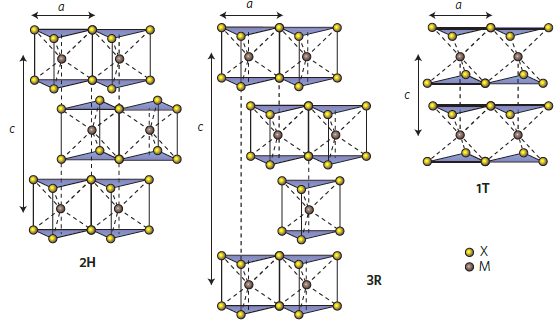
\includegraphics[scale=0.7]{TMDCPolytypes.png}
	\caption{Schematics of the structural polytypes: 2H (hexagonal symmetry, two layers per repeat unit, trigonal prismatic coordination), 3R (rhombohedral symmetry, three layers per repeat unit, trigonal prismatic coordination) and 1T (tetragonal symmetry, one layer per repeat unit, octahedral coordination). The chalcogen atoms (X) are yellow and the metal atoms (M) are grey. The lattice constants a are in the range 3.1 to 3.7 Å for different materials. Adopted from \cite{ElectronicsAndOptoelectronicsOfTwo-dimensionalTransitionMetalDichalcogenides}}
	\label{fig:TMDCPolytypes}
	\end{center}
	\end{figure}
	
	Since graphene have proven to be difficult to work with in the fields of semiconductors due to its lack of natural finite electronic band gap its role as a successor in electronic and opto-electronic devices remains to be seen. However the techniques learned and effects observed during its characterisation were easily transferred to other layered compounds such as TMDCs. In particular the semiconducting, group VI-based TMDCs, containing sulphur and selenium as chalocgen atoms have proven to be more readily potentially useful as an active material in electronic and opto-electronic devices. This is due to their inherent electronic and optical bandgap in visible-near IR range. 
	
	As the number of layers changes from bulk to monolayer the properties of the TMDC undergo a significant change. In most TMDCs the bandgap changes from indirect to a larger direct one. 
	
	\subsection{Electronic properties}
	\label{subsec:Electronic properties}
	
	One of the most interesting features that the layered TMDC materials exhibit is the shift in the bandstructure with the changing number of layers. Several studies have shown in simulations and experimentally that TMDCs have very similar electronic band structure as seen in example of $WS_2$ in Figure \ref{fig:WS2BandStructureSimulation}. In bulk $WS_2$ the maximum of the valence band (VBM) at $\Gamma$ point and the minimum of the conduction band (CBM) at $\Lambda$ form an indirect bandgap. As the number of the layers decreases the CBM at $\Lambda$ point as well as VBM at $K$ point increases causing the band gap to widen. At 2 layers the $K$ point becomes the actual CBM and a new indirect bandgap forms between $\Gamma$ point and $K$ point. Finally in a $WS_2$ monolayer the VBM at $K$ point as well as entire conduction band increases to form a new greater direct band gap at $K$ point. This means that $WS_2$ bandgap changes from 1.3 eV indirect bandgap in bulk to 2.1 eV direct bandgap in monolayer.
	
	\begin{figure}[h]
	\begin{center}
	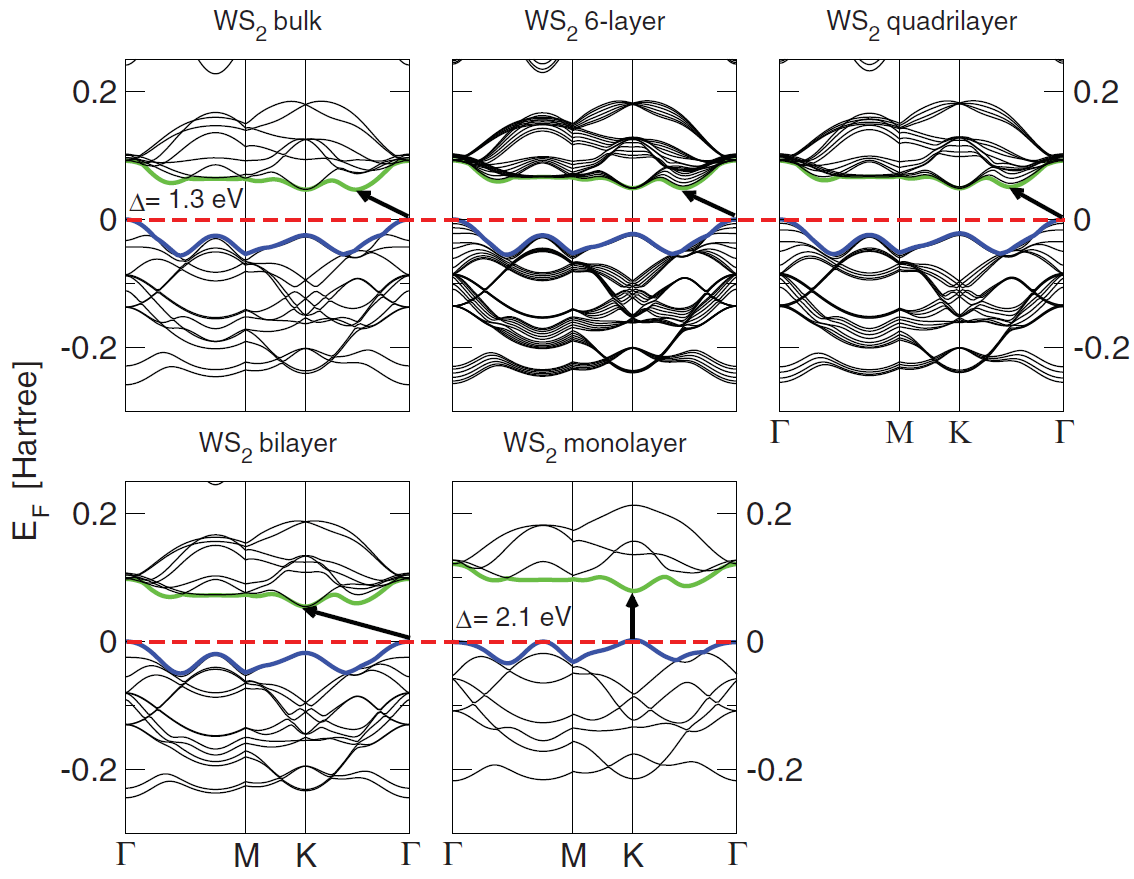
\includegraphics[scale=0.4]{WS2BandStructureSimulation.png}
	\caption{Band structures of bulk $WS_2$, its monolayer, as well as, polylayers calculated from the density functional theory (DFT) simulation. The horizontal dashed lines indicate the Fermi level. The arrows indicate the fundamental band gap (direct or indirect) for a given system. The top of valence band (blue) and bottom of conduction band (green) are highlighted. Adopted from Ref. \cite{WS2BandStructureSimulation}}
	\label{fig:WS2BandStructureSimulation}
	\end{center}
	\end{figure}
	
	Like $WS_2$ other Mo and W based TMDC undergo similar transitions as seen in Table \ref{tab:MoWBandgapsComparison}. In all cases the smaller indirect bandgap changes to greater direct bandgap with monolayer bandgap ranging from 1.1 eV to about 2.1 eV. Moreover the VBM at K points exhibits the orbit-spin band splitting at the K point of about 400 meV. This direct bandgap leads to presence of A and B excitons generated by transition between CBM and two VBMs at the K point. The conduction band as well as the valence band are dominated by the d-electron orbitals of the transition metal atoms and at the VBM and CBM they hybridize with the p-electron orbitals of the chalcogenide atoms. Because the hybridization happens mostly at the $\Gamma$ point and the chalcogenide atoms are at the surface of the TMDC layer it leads to strong interactions between the layers. This leads to significant change in the band structure at the $\Gamma$ and rise of the indirect bandgap as a result of increased number of layers. On the other hand at the $K$ point the d-orbitals of the transition metals remain mostly unaffected due to them being positioned in the middle of the layer \cite{WS2BandStructureSimulation} \cite{EmergingPhotoluminescenceInMonolayerMoS2}
	 
	 \begin{table}[h]
	 \caption{Mo and W based TMDC bandgaps comparison}
	 \label{tab:MoWBandgapsComparison}
	 \end{table}
	 
	 \begin{center}
	 \begin{tabular}{c|l|l|l}
	 
	 M$\backslash$X & $-S_2$ 			& $-Se_2$ 	& $-Te_2$\\ \hline
	 $Mo$ 			& Semiconducting	& Semiconducting	& Semiconducting	\\ 
	 				& 1L:1.8 eV			& 1L: 1.5 eV		& 1L: 1.1 eV		\\
	 				& Bulk: 1.2 eV		& Bulk: 1.1 eV		& Bulk: 1.0 eV		\\ \hline
	 W 				& Semiconducting	& Semiconducting	& Semiconducting	\\
	 				& 1L:2.1 eV			& 1L: 1.7 eV		& 1L: 1.1 eV		\\
	 				& Bulk: 1.4 eV		& Bulk: 1.2 eV		& 					\\
	 
	 \end{tabular}
	 \end{center}
	
	
	\subsection{Optical properties}
	\label{subsec:Optical properties}

	TMDCs exhibit a wide array of opto-electronic effects due to their strong light-matter effects. These effects are mostly caused by the abundant presence of excitons, bi-excitons, trions or bound excitons. As a result the change in layer thickness from bulk to monolayer alters the photoluminescence, photoconductivity and absorption in the visible to infrared range.
		
	The primary and most common quasi-particle that forms in such system is an exciton, which is a pair of a negatively charged electron and a positively charged hole bound together by Coulomb forces to form a structure similar to that of hydrogen atom. Such pair is electrically neutral and is of size exceeding size of single cell which makes it a Wannier–Mott exciton. The recombination of these excitons results in a photon emission which can be easily observed during photoluminescence characterisation. On top of excitons other quasi-particles such as trions, bi-excitons or bound excitons can be found. A trion is a group of 2 electrons and a hole or 2 holes and an electron, or otherwise described as a charged exciton. The exact nature of the trion depends usually on the type of intrinsic doping of the TMDC. A bi-exciton is a pair of excitons which is usually only observed in quantum dot systems but can be also seen in excitonically dense systems such as TMDCs. A bound exciton is similar to the free exciton but is trapped by a defect. In a typical photoluminescence spectrum several peaks can be observed depending on specific type of TMDC characterised. In $WS_2$ monolayer for instance as seen in Figure. \ref{fig:WS2TypicalPLSpectra} the strongest peak (often labelled as an A peak) at about 1.97 eV is caused by the direct transition of single-photon generated exciton. Slightly redshifted by about 30 meV from the A peak a generally weaker peak caused by the trion recombination can be found. At higher energies another peak can be observed due to the presence of bi-excitons. At around the 1.3 eV a much weaker peak (I) can be seen caused by the indirect transition. Additionally a B peak can be observed blueshifted from the A peak which is caused by valley splitting as discussed in chapter \ref{subsec:Electronic properties}. As seen in Figure \ref{fig:WS2TypicalPLSpectra} as the number of layers increases the main A peak becomes dramatically weaker due to lack of direct transition and redshifted following the pattern discussed in chapter \ref{subsec:Electronic properties}. At the same time the I peak becomes relatively stronger and eventually dominates the bulk material.
		
	\begin{figure}[h]
	\begin{center}
%	\includegraphics[scale=1]{•}
	\caption{Typical PL spectra of $WS_2$}
	\label{fig:WS2TypicalPLSpectra}
	\end{center}
	\end{figure}
		
	Similarly the photoconductivity of the TMDCs is strongly reliant on the number of layers and incident photon energy. The $MoS_2$ for instance shows 3 times stronger photoconductivity in monolayer around 1.8 eV, where the direct transition is located, than in 2L $MoS_@$ around 1.6 eV. Additionally the photoconductivity appears to increase in steps with relation to the photon energy following the direct and indirect transitions. \cite{ElectronicsAndOptoelectronicsOfTwo-dimensionalTransitionMetalDichalcogenides}.
		
	The sunlight absorption in TMDCs has been shown to be significantly more intense than in commonly used solar cell materials, at about 5-10$\%$ which is an order of magnitude greater compared to similar thickness of Si or GaAs. It is also stronger compared to 2-3$\%$ of sunlight absorption of graphene. As a result a excitonic solar cell based on $MoS_2/WS_2$ bilayer shows about 1$\%$ power efficiency, about 3 times greater than that of typical ultrathin solar cells \cite{ExtraordinarySunlightAbsorptionAndOneNanometerThickPhotovoltaicsUsingTwo-DimensionalMonolayerMaterials}.
	
	During standard single photon excitation photoluminescence studies the excitons generated can be called "bright" since they appear in PL spectrum. The reason we can observe them easily is because the spin between an electron and a hole is conserved, and thus allowing for photon emission. However another combination is possible, called dark exciton, where both electron and the hole have the same spin. Because of that they cannot recombine by emitting a photon and therefore remain absent from the PL spectrum. Even though they exist much longer than their bright counterparts their presence is of course also more difficult to observe. One way to observe them is to use two photon excitation. Due to two photon selection rule the single photon excitation can be excluded and the dark excitonic states can be observed. In WS2 the dark excitons result in two peaks at 2.28 eV and 2.48 eV. [Probing excitonic dark states in single-layer tungsten disulphide]
	
	Defect engineering allows to tune the number of charge carriers. In MoS2 or WS2 the sufur vacancies lead to increased number of electrons in the material. Because of that by increasing the number of defects in those materials the level of n-doping can be changed. An easy way to observe the presence of those defects and subsequent quenching of them is to expose the material to varying amounts of oxygen, nitrogen or water. Due to greater electronegativity (???) those species attract the electrons and therefore the electron population in the material decreases. This in turn leads to smaller trion population since trions require an extra electron to form. This then can be observed in PL as a more narrow direct peak, with especially smaller redshifted shoulder. The effect can also be of course reversed by decreasing the amount of oxygen, nitrogen or water in the environment since those exist in already in ambient conditions [Optical control of charged exciton states in tungsten disulfide].
	
	In order to introduce and control the amount of vacancies in the TMDC different method have to be explored. One of the ways of achieving that in already grown material is the use of oxygen plasma. It has been shown that the number of defects can be controlled by limiting the plasma exposure. During the process the oxygen also chemically bonds to the MoS2 at the defect sites and therefore partially negates the effect of defects on the optical properties. The PL can also be seen to increase in intensity with increasing number of defects with oxygen adsorped due to the increased yield of bound excitons localised at these defects. [Strong Photoluminescence Enhancement of MoS2 through Defect Engineering and Oxygen Bonding]
	
	Similar effect has been shown using the 2,3,5,6-tetrafluoro-7,7,8,8-tetracyanoquinodimethane ($F_4TCNQ$), 7,7,8,8-tetracyanoquinodimethane ($TCNQ$) and (nicotinamide adenine dinucleotide) $NADH$ for chemical doping. Both $F_4TCNQ$ and $TCNQ$ are p-type dopants while $NADH$ is a n-type dopant. By exposing the surface of MoS2 to these compounds the change in PL intensity and FWHM have been observed. Similar to doping with $O_2$, $N_2$ or $H_2O$, all of which are p-type dopants, the intensity of PL has increased in presence of $F_4TCNQ$ and $TCNQ$. The effect has been similarly ascribed to lowering the number of defects and therefore the lowering the trion population and subsequently increasing the exciton population increasing the yield. The opposite observation has been made with use of $NADH$ with PL intensity decreasing. Similarly the increase in trion population with lower PL yield is ascribed to the lower PL intensity. [Tunable Photoluminescence of Monolayer MoS2 via Chemical Doping].
	
	It has also been show that alloying can be used to fine tune the PL by varying the concentration of alloying material. In monolayer $Mo_{1-x}W_xS_2$ the PL peak position initially decreases from 1.575 eV (PL peak position of pure MoS2) to 1.56 eV at x=0.21 and then increase up to 1.65 eV (PL peak position of WSe2) at x = 1. This effect could be attributed to the linearity of VB and non-linearity of CB with regards to change in W composition. The PL position can therefore be engineered on a monotonic range from 1.56 eV to 1.65 eV. In bilayer $Mo_{1-x}W_xS_2$ alloy the position of both direct and indirect transition PL peaks increases monotonically from about 1.49 eV and 1.53 eV for pure MoSe2 to 1.56 eV and 1.62 eV for pure WSe2 as the W amount is increased. This opens another relatively easy way of engineering PL position [Two-Dimensional Molybdenum Tungsten Diselenide Alloys: Photoluminescence, Raman Scattering, and Electrical Transport].
	
	Another effect that has been demonstrated that allows for certain degree of control of PL in TMDCs is relation between the helicity of incident light and valley population valley population. It has been shown that by exciting the monolayer $MoS_2$ with right-polarised light the resulting excitons will fill primarily the VB at K point. Similarly by exciting the $MoS_2$ with left-polarised light the excitons will fill the VB at K' point. After recombination the resulting photons will exhibit the same circular polarity as the photons that excited the electrons in the first place. [Tightly bound trions in monolayer MoS2] [Control of valley polarization in monolayer MoS2 by optical helicity]
	
	The temperature effect on TMDCs has also been investigated. In $WSe_2$ monolayer it has been shown that as the temperature of the sample increases from room temperature to about 400K the position of the direct transition PL peak redshifts from about 1.65 eV to about 1.58 eV. When the temperature is decreased from room temperature to about 5K the same peak blueshifts to about 1.7 eV. Between 100K and 50K as well 20K and 5K the position of the PL peak does not change. Additionally around 120K another peak appears and as the temperature is lowered it also blueshifts although less than the RT peak. The peak only present at RT is attributed to free excitons whereas the peak appearing at 120K is ascribed to bound excitons. As bound exciton peak appears its intensity increasese with lower temperature while the intensity of the free exiton peak decreases. This indicates that the population of free excitons decreases while the population of the bound excitons increases with decreasing temperature \cite{PhotoluminescencePropertiesAndExcitonDynamicsInMonolayerWSe2}
	
	There has been many reports on the spatial distribution of PL in the TMDCs. One of the observed patterns in WS2 and MoS2 has been that of much stronger PL intensity at the edges of the flakes. That effect has been primarily observed in small flakes of about 5 $\mu m$ \cite{ExtraordinaryRoomTemperaturePhotoluminescenceInTriangularWS2Monolayers}.
	
	\subsection{Phonon dispersion}
	
	The vibrational and phononic characteristics of TMDCs have been investigated at length by both theoretical simulations as well as experimental studies. The $2H-MX_2$ crystal structure of the TMDCs belongs to $D_{6h}^4$ point group and there are 18 lattice dynamical modes at the $\Gamma$ point. Phonons belonging to these modes can be represented as Eq. \ref{eq:PhononDispersionRepresentation} \cite{LatticeDynamicsInMono-AndFew-LayerSheetsOfWS2AndWSe2}: 
	
	\begin{equation}
	{\Gamma} = A_{1g} + 2A_{2u} + B_{1u} + 2B_{2g} + E_{1g} + 2E_{1u} + E_{2u} + 2E_{2g}
	\label{eq:PhononDispersionRepresentation} 
	\end{equation}
	
	In TMDCs 4 active Raman modes can be observed $E_{1g}, E^1_{2g}, E^2_{2g}, A_{1g}$. These can be seen in Figure \ref{fig:4ActiveRamanModes}. The $E^2_{2g}$ is a shear mode that involves 2 layers vibrating against each other. The $E_{1g}$ is an in-plane vibration of chalcogen atoms but is forbidden in the back-scattering configuration. For monolayers therefore it leaves primarily the $E^1_{2g}$ which is an in-plane mode involving vibration of both metal and chalcogen atoms as well as $A_{1g}$ which is an out-of-plane mode involving only chalcogen atoms. 
	
	\begin{figure}[h]
	\begin{center}
	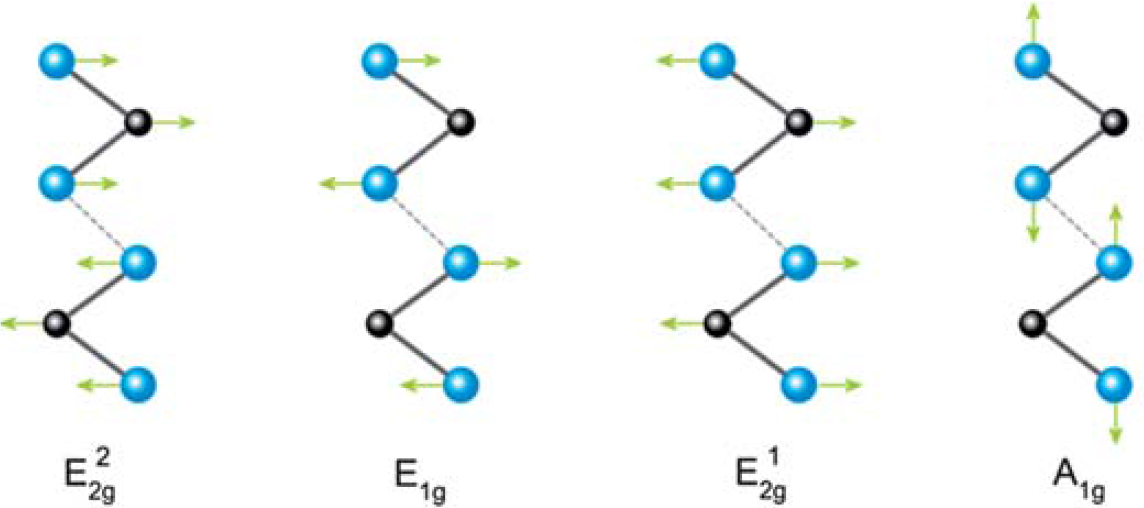
\includegraphics[scale=0.4]{RamanActiveModes.png}
	\caption{4 active Raman modes in TMDCs. Metal atoms and chalcogen atoms are black and blue respectively. Adopted from \cite{LatticeDynamicsInMono-AndFew-LayerSheetsOfWS2AndWSe2}}
	\label{fig:4ActiveRamanModes}
	\end{center}
	\end{figure}
	
	These two peaks tend to dominate the spectrum of any TMDCs, whether monolayer or few-layer or bulk. The shear mode $E^2_{2g}$ appears at low Raman shift frequencies and is therefore difficult to observe but can be used to differentiate monolayer from few-layer material. Since $E^1_{2g}$ is an in-plane mode it tends to be unaffected by the number of layers due to weak van der Vaals forces between the layers but can be seen to be slightly redshifted as the number of layers increases. As seen in Figure \ref{fig:TypicalRamanSpectrumWS2} the $E^1_{2g}$ peak at about 352 $cm^{-1}$ is overlapping with another stronger peak, a 2LA(M) peak at 350 $cm^{-1}$ which is a longitudinal acoustic mode caused by in-plane collective oscillations of W and S atoms. The second strongest peak at around 416 $cm^{-1}$ is an $A_{1g}$ peak, caused by out of plane vibrations. Because of that it is much more sensitive to the number of layers and is seen to become blueshifted as the number of layers increases. This has been attributed to the restorive forces as well as increase in dielectric screening of the Coulomb forces. Combining both of these shifts in frequency with the changing number of layers the difference between these two peak position can be used to identify the number of layers in TMDCs as seen in Figure \ref{fig:LayerNumberIdentificationRamanShiftWS2}
	
	\begin{figure}[h]
	\begin{center}
%	\includegraphics[scale=1]{•}
	\caption{Typical Raman spectrum of $WS_2$}
	\label{fig:TypicalRamanSpectrumWS2}
	\end{center}
	\end{figure}
	
	\begin{figure}
	\begin{center}
%	\includegraphics[scale=•]{•}
	\caption{Identification of number of layers by the difference in position of $A_{1g}$ and $E^1_{2g}$ peaks.}
	\label{fig:LayerNumberIdentificationRamanShiftWS2}
	\end{center}
	\end{figure}
	
	\subsection{Heterostructures}
	\subsection{Applications}
\section{Methods}
	\subsection{Raman spectroscopy theory}
	\subsection{Photoluminescence spectroscopy theory}
	\subsection{XPS theory}
	
\section{Role of precursors in growth of monolayer $WS_2$}
	\subsection{Introduction}
	
Monolayers of transition metal sulphides and selenides exhibit range of interesting properties such as strong light absorption in the IR and visible range \cite{AtomicallyThinMoS2ANewDirect-GapSemiconductor}\cite{ExtraordinarySunlightAbsorptionAndOneNanometerThickPhotovoltaicsUsingTwo-DimensionalMonolayerMaterials}\cite{EvolutionOfElectronicStructureInAtomicallyThinSheetsOfWS2AndWSe2}, valley polarisation \cite{ControlOfValleyPolarizationInMonolayerMoS2ByOpticalHelicity} \cite{ValleyPolarizationInMoS2MonolayersByOpticalPumping}, spin-orbit interactions \cite{CoupledSpinAndValleyPhysicsInMonolayersOfMoS2AndOtherGroup-VIDichalcogenides}\cite{GiantSpin-orbit-inducedSpinSplittingInTwo-dimensionalTransition-metalDichalcogenideSemiconductors}, tightly bound excitons \cite{TightlyBoundTrionsInMonolayer} or second-harmonic generation \cite{ProbingSymmetryPropertiesOfFew-LayerMoS2Andh-BNByOpticalSecond-HarmonicGeneration}. Some of these effects can be attributed to the lack of free dangling bonds and configuration of d-orbitals \cite{TheTransitionMetalDichalcogenidesDiscussionAndInterpretationOfTheObservedOpticalElectricalAndStructuralProperties}, \cite{ElectronicPropertiesOfMoS2Nanoparticles}.

Among these materials one of the most promising is the $WS_2$. Its visible range bandgap of 2eV as well as an easy and safe manufacturing route via CVD makes it one of the more interesting and studied TMDCs. The typical characterisation by photoluminescence spectroscopy allows to probe the varying synthesis conditions, the grain boundaries or defect population \cite{ExtraordinaryRoomTemperaturePhotoluminescenceInTriangularWS2Monolayers} \cite{doi:10.1021/nn4046002} \cite{Li2015} \cite{Rong2014}. The PL efficiency in as-grown monolayer $WS_2$ produced via CVD growth shows {$\sim$}2-6\% efficiency \cite{doi:10.1021/nn4046002}\cite{Yuan2015} \cite{doi:10.1021/nn403682r}. This efficiency is caused mostly by defect-mediated non-radiative recombination centres \cite{Amani2015}. LEDs have been successfully produced \cite{doi:10.1021/nl500171v} showing external quantum efficiency up to 10\% \cite{Zeng2016}\cite{Withers2015}. $WS_2$ is typically a n-type semiconductor due to the presence of sulphur vacancies \cite{ExtraordinaryRoomTemperaturePhotoluminescenceInTriangularWS2Monolayers}\cite{doi:10.1021/nn5059908}\cite{Iqbal2015}. In order to utilise this material in any potential future applications a reliable and scalable manufacturing method must be developed to ensure a high quality crystal on the wafer scale area. The main method for $WS_2$ synthesis that satisfies these conditions is Chemical Vapour Deposition (CVD) \cite{Hofmann1988}. The growth of tungsten based TMDCs have been less successful than the equivalent molybdenum based TMDCs and has produced mostly isolated flakes of up to 40 $\mu m$ \cite{ExtraordinaryRoomTemperaturePhotoluminescenceInTriangularWS2Monolayers} \cite{doi:10.1021/nn403454e} \cite{Rong2014} \cite{doi:10.1021/nn400971k}\cite{doi:10.1021/acsnano.5b01480}\cite{Fu2015}\cite{Lee2013}. Even larger films of monolayer $WS_2$ have been shown, however they also exhibit low carrier mobility \cite{Kang2015}\cite{Gao2015}. In the typical CVD synthesis process the sulphur and tungsten oxide are evaporated simultaneously in a tubular furnace with a constant flow of carrier gas like argon at temperatures of at least 900 {\degree}C \cite{ExtraordinaryRoomTemperaturePhotoluminescenceInTriangularWS2Monolayers}\cite{doi:10.1021/nn403454e}\cite{Rong2014}\cite{doi:10.1021/nn400971k}\cite{doi:10.1021/acsnano.5b01480}\cite{Fu2015}\cite{Lee2013}. Such growth is predicated by topotacic transformation leading to low density distribution of domains on an amorphous \cite{ExtraordinaryRoomTemperaturePhotoluminescenceInTriangularWS2Monolayers}\cite{doi:10.1021/nn403454e}\cite{doi:10.1021/nn400971k}\cite{Fu2015}\cite{Lee2013} or crystalline substrate \cite{Rong2014}\cite{doi:10.1021/acsnano.5b01480}\cite{doi:10.1021/nn503093k} possibly due to low evaporation rates of $WO_3$. Since $WO_3$ requires high temperatures of 950-1000 {\degree}C to evaporate while the $S$ becomes volatile at 90 {\degree}C the thermodynamics of the process are difficult to control. The low growth dictated by fast evaporation of $S$ leads to limited domain growth and lack of continuous layer. One of the proposed solutions have been to spread the $WO_3$ on the target substrate \cite{doi:10.1021/nn4046002}\cite{Li2015}\cite{Gao2015}\cite{Cong2013}\cite{Yun2015}\cite{Gong2015}\cite{Gong2014}. This has however led to low reproducibility, poor control of thickness and stoichiometry and unreacted material left on the substrate. Another approach has been to use more volatile $W$ precursors such as $WCl_6$\cite{Carmalt2003} or $W(CO)_6$\cite{Kang2015}\cite{Eichfeld2015} together with organic compounds as $S$ precursors. Such method while producing a large area domains at lower temperature has led to lower crystal quality and purity.

Here we propose a different method of CVD synthesis that allows for much larger flake growth of up to 800 $\mu m$ at temperature of 750 {degree}C. Such grown material exhibits high electron mobility in one and two layers of $WS_2$, higher than other values reported in literature. The photoluminescence peak is also very narrow at 36 meV FWHM at room temperature. 

	\subsection{Results}
	
For the purpose of comparing the CVD synthesis method conditions the several sets of precursors were used: $WO_3$, $WO_3$ + NaCl and $H_2WO_4$ + NaCl.


%  paper


RESULTS
The synthesis of WS2 was performed starting from commercial powders of H2WO4, WO3, S and where indicated, we have introduced NaCl. W and S precursors were placed in two separate crucibles well-spaced in a quartz tubular furnace (Supplementary Information, Figure S1a) and heated up independently using different controllers as reported in Figure S1b. The heating profile of S has been optimized to ensure maximum supply when the W-precursors start evaporating. SiO2 (285 nm)/Si substrates were utilized for the growth and loaded in the downstream zone of the tubular furnace. This approach allows for a controllable and reproducible large-area deposition of uniform WS2 domains compared to placing the substrate above the metal precursor crucible. The syntheses were carried out under low vacuum and a flux of Ar gas. Optical micrographs of WS2 monolayers (Figure 1) grown by using different W precursors (WO3, WO3-NaCl and H2WO4-NaCl) at different temperatures (950 {\degree}C, 850 {\degree}C and 750 {\degree}C) show distinctively increasing lateral size of the triangles and increasingly facilitated synthesis at lower temperatures from the left to the right side of the figure. For all of the growth conditions, we observe that the WS2 triangles present sharp edges and uniform colour contrast onto SiO2, suggesting formation of pristine monolayer WS2 across the entire triangle area. WO3 precursor growth leads to monolayered WS2 triangles with lateral size of {$\sim$}10 {$\mu$}m at 950 {\degree}C (Figure 1a) while no deposition of WS2 is observed at lower temperatures (850 {\degree}C and 750 {\degree}C) (Figure 1b, c). The fact that the synthesis can occur only at very high temperature is explained by the high sublimation temperature of WO3.  
 
Figure 1 Optical micrographs of WS2 triangles grown on SiO2/Si substrates at different temperatures and using different precursors: (a) WO3 at  950 {\degree}C; (b) WO3 at 850 {\degree}C; (c) WO3 at 750 {\degree}C; (d) WO3 and NaCl at 950 {\degree}C; (e) WO3+NaCl at 850 {\degree}C; (f) WO3 + NaCl at 750 {\degree}C, the OM appears as a bare SiO2 substrate; (g) H2WO4 + NaCl at 950 {\degree}C; (h) H2WO4 and NaCl at 850 {\degree}C; (i) H2WO4 + NaCl at 750 {\degree}C.
                                        
The WO3+NaCl system overall facilitates the synthesis of WS2 triangles leading to {$\sim$}60 {$\mu$}m flakes at 950 {\degree}C (Figure 1d) and {$\sim$}30 {$\mu$}m (Figure 1e) at 850 {\degree}C. The larger WS2 domains obtained at higher temperatures can be explained in the light of the Robinson \& Robin model [ ]. At high temperature the diffusivity of the adsorbed precursors on the SiO2 surface is favourable leading to the expansion of the existing domains. At the same time the desorption of absorbed species is higher than at lower temperatures, limiting the achievement of a supersaturation concentration and thus reducing the nucleation density. By further lowering the growth temperature to 750 {\degree}C, no WS2 domains have been observed (Figure 1f) likely due to the insufficient evaporation of WO3.                                                                                              By replacing WO3 with H2WO4 the lateral size of the WS2 monolayered domains significantly increases (Figure 1g,h,i). The triangular crystals have edge lengths exceeding 200 {$\mu$}m at temperatures higher than 850 {\degree}C and between 50-200 {$\mu$}m at 750 {\degree}C (Figure 1g,h,i). Continuous polycrystalline monolayer coverage has been obtained over areas of {$\sim$}0.8 mm extension (Figure S2). Increasing the growth pressure (from 1.6 mbar to 13 mbar) at 950 {\degree}C bilayered WS2 flakes are preferentially formed (Figure S3). To understand the facilitated synthesis of WS2 using H2WO4 and NaCl, we conducted X-ray diffraction (XRD) analysis of the reaction products between H2WO4+NaCl and WO3+NaCl systems at different temperatures (500 {\degree}C, 650 {\degree}C and 750 {\degree}C) to understand the chemical differences (Figure S4). We found that the main products of the reactions between NaCl and H2WO4 are: NaxWyOz and tungsten oxychloride (WClO4 and WO2Cl2). The NaxWyOz possesses a high evaporation temperature as it remains in the crucible (Figure S5) after the synthesis of WS2 is completed. Further, using this compound as precursors for a new growth of WS2 at 950 {\degree}C did not lead to the formation of any WS2 flakes, confirming the high evaporation temperature. On the bases of previous studies on the synthesis of bulk crystals, the formation of tungsten oxychloride species (WO2Cl2 and/or WOCl4) is likely to occur while the formation of metal halides is less favourable (e.g. WCl6) [ ][ ]. Tungsten oxychlorides are volatile already at 200 {\degree}C [ ] and they can be sulfidized in vapour phase and then be deposited onto the target substrate as atomic clusters. WOCl4 has been previously used [43] as precursor for the CVD synthesis of WS2 bulk films. Despite its strong tungsten oxygen double bonds, WOCl4 proved to be an effective precursor with a clean decomposition pathway in the CVD process without formation of tungsten oxysulfide. We have verified that using this precursor is indeed possible to obtain WS2 at temperatures as low as 550 {\degree}C (Figure S6a). The key role played by the oxyhalide species it becomes apparent if we try to grow WS2 by using only hydrated tungsten oxide. As this decomposes to form WO3, only small WS2 domains are observed with similar PL characteristics to the WO3 precursors-growth (Figure S6b). Furthermore, to confirm the key role played by Cl, we replaced NaCl with KCl and we obtained comparable growth results (Figure S6c).
High resolution TEM imaging confirms the pure crystalline nature of the material (Figure 2a). The measured lattice constant is 0.3 nm consistent with that of 2H-WS2 (a=0.318 nm). The AFM thickness profile analysis of WS2 triangles confirms the monolayer (Figure 2b,c) and bilayer (Figure S3d,e) nature of the flakes. This shows an edge step height of {$\sim$}0.8 nm which confirms the monolayer nature of the WS2 domains [ ][ ].                                                                                                                               
The Raman spectra of WS2 obtained under the different growth conditions are shown in Figure 2d. All of the spectra exhibit two characteristic peaks located at {$\sim$}(351{$\pm$}0.53) cm−1 and {$\sim$}(417.6{$\pm$}1) cm−1, which can be attributed to 2LA-E12g and A1g Raman modes of pristine WS2 monolayer [ ][ ]. Interestingly the distribution of the peak positions is increasingly narrower going from WO3 precursor, to WO3+NaCl and to H2WO4+NaCl (Figure S8, S10). The Raman peak intensities are uniform across the entire triangle area (Figure S7, S9) and the energy difference (${\Delta}{\nu}$) between 2LA(M) and A1g is {$\sim$}(66.5{$\pm$}0.53) cm−1 (Figure S11), as expected for WS2 monolayers [51].   
 
Figure 2 Structural and physical characterization of WS2 triangles: (a) HRTEM image of the WS2 lattice grown using H2WO4+NaCl, the inset report a selected diffraction area which show a hexagonal pattern. (b) Raman spectra showing the characteristics active modes of WS2 grown under different conditions and compared with mechanically exfoliated flakes. (c) AFM image and (d) corresponding thickness profile of monolayer WS2.
A comparison of representative photoluminescence (PL) intensity maps of WS2 monolayers grown by using the three precursor systems at different temperatures is reported in Figure 3. The PL intensity map of WS2 monolayers grown at 950 {\degree}C from WO3 (Figure 3a) shows a three-lobes intensity pattern. The PL spectra appear asymmetric and they can be deconvolved in two distinct peaks which have been attributed to an exciton and a trion component (Figure 4a) [ ]. The PL peak positions of the same WS2 flake show a bimodal distribution with areas with high PL intensity distributed over three lobes characterized by a peak position distribution centred at 1.94 eV versus areas with low intensity and peak position centred at 1.96 eV. The FWHM is centred at 75 meV versus 55 meV respectively in the two areas (Figure 4a-c) (Figure S12, S13, S15). Peak position and FWHM are comparable with the current state-of-the-art of WS2 synthesis from WO3 [4][18][ ][ ]. The red shift of {$\sim$}0.02 eV of the peak position (Figure 4b) and the larger FWHM (Figure 4c) of the three-lobe areas suggests higher concentration of structural defects [ ][59]. In particular in the form of S-vacancies which increases the electron density and consequently the trion population [4][ ]. This leads to the strengthening of PL emission at lower energies than the optical band gap (Figure 4) causing a redshift and an increased FWHM of the peak [4][57]. Strain variations in the lattice can also affect the light emission intensity and wavelength [ ][ ]. To prove whether lattice strain could affect the PL energy and the intensity variation, we have relaxed the lattice by cutting the WS2 domain using a high intensity 532 nm laser. As reported in Figure S14, the PL peak intensity and energy position patterns remain unchanged along with the Raman peak position. Thus, structural defects in variable concentration are likely to be the main responsible for the PL intensity and peak position pattern [ ]. The samples grown with the addition of NaCl present light emission at higher energy and FWHM narrower compared to the WO3-led growth. The PL spectra appear asymmetric and they can be deconvolved in two distinct peaks which have been attributed to an exciton and a trion component (Figure 4a). The distribution of the PL peak position and FWHM is uniform within the same triangle but bimodal with respect to different triangles and they possess small standard deviations (Figure 4b-c) (Figure S12, S13, S16) compared to the WO3-led growth. The light emitted has higher energy ({$\sim$}1.95{$\pm$}0.002 eV and 1.96{$\pm$}0.002 eV) and the FWHM of the peaks is narrower ({$\sim$}43{$\pm$}2.8 meV and 51{$\pm$}3 meV) (Figure 4), compared to WO3-led growths and most of the reported works [4][18][54][55]. This suggests that the trions component is now reduced. Thus we can conclude that WS2 grown form NaCl+WO3 is affected by less structural defects compared with WO3-growth. A different growth dynamics (topotactic versus molecular conversion) which leads to a different distribution of defects can explain the differences observed (Figure 3b-c). 
 
Figure 3 Spatial maps of PL intensity of WS2 grown in the conditions exemplified in Figure 1. The scale bar length is 10$\mu$m.
The overall PL peak intensity of WS2 monolayers (Figure 3d-f) grown using H2WO4+NaCl is considerably higher compared to the previously discussed growth systems. Further, the FWHM is significantly narrower ({$\sim$}36{$\pm$}3 meV), and the PL energy ({$\sim$}1.980{$\pm$}0.005 eV) is higher compared to FWHM and emitted light observed for WS2 grown under WO3 and WO3+NaCl precursors (Figure 4) (Figure S12, S13, S17). This suggests that the material grown by using H2WO4+NaCl possess even less structural defects and particularly in the form of sulfur vacancies, which lead to a negligible contribution from trions (Figure 4a). Further, no appreciable differences are observed from flake to flake, confirming the high reproducibility of the process. The FWHM is smaller than previously reported values for CVD-grown [4][18][54][55] and exfoliated WS2 [6][ ] (Figure 4a) while it is comparable to WS2 grown on van der Waals substrates [38] and to high quality exfoliated WS2 [22]. Overall the distribution of the PL peak position and the FWHM for the samples grown introducing H2WO4 are much narrower (5 meV and 3 meV respectively) (Figure S18) compared with the other precursors results. Different intensity patterns across individual flakes can still be recognized, however, they present smaller intensity difference compare to the other growth conditions. 
 
Figure 4: PL spectra characteristics of WS2 grown using: WO3 at 950 {\degree}C, WO3+NaCl at 850 {\degree}C, H2WO4+NaCl at 850 {\degree}C: (a) individual spectra (dotted line) and deconvolution in exciton and trion components; (b) distribution of PL peak position and (c) distribution of PL FWHM for several WS2 grown using the three different precursor systems.
XPS characterization confirms the greater efficiency of tungstic acid in inducing a complete sulfidization of the precursors compared with the WO3+NaCl system. Analysing WS2 grown using H2WO4+NaCl, the W 4f5/2 and W 4f7/2 core levels (Figure 5a) present peak position characteristic of W4+ in WS2 [ ][ ] (32.7 and 34.8 eV respectively) and the narrowest achievable FWHM (1 eV) (Figure 5a), using the Mg K$\alpha$ as X-ray source. This indicates chemical purity and perfect stoichiometric ratio of W and S. This has been also confirmed by calculating the concentration of S and W from the integrated intensity of the W 4f and S 2p core levels. The S 2p1/2 and 2p3/2 core levels, also appear at the expected position for WS2 (162.3 eV and 163.4 eV respectively, Figure 5b) [63] and with a very narrow FWHM (1 eV) (Figure 5c). A very small amount of W6+ (W 4f5/2 and W 4f7/2 core levels centred at 35.9 eV and 38.1 eV respectively in Figure 5a) attributable to WO3, which partially overlaps with the W 5p core level (38.5 eV), can be observed which however disappears after transferring the flakes on a new SiO2/Si substrate (Figure 5c) and thus suggesting that it is related to residual precursors on the substrate considering the XPS spot size is {$\sim$}1 mm. It is worth noting that after transfer the FWHM of the W 4f core levels remains unchanged suggesting that the transfer process preserves the crystallinity of the flakes and no additional defects are introduced.
Similarly, chemical purity and expected stoichiometric ratio of 2:1 for S:W have been observed for WS2 grown from WO3+NaCl (Figure 5a). Nevertheless, a larger W6+ contribution, attributable to WO3  (W 4f5/2 and W 4f7/2 centred at 35.9 eV and 38.1 eV respectively in Fig 5a) has been detected in this case suggesting that a conspicuous amount of precursors does not get sulfurized and it is just deposited onto the SiO2 wafer. Upon transfer on a new SiO2/Si substrate, this component entirely disappears (Figure 5c), thus indicating also in this case that WO3 is mainly distributed on the substrate. The FWHM of the W4+ 4f core levels is {$\sim$} 1.2 eV in this case, suggesting higher concentration of defects compare to H2WO4+NaCl-led growth (Figure 5a). The transferred WS2 present a FWHM even larger {$\sim$}1.3 eV, suggesting the introduction of atomic defects as a consequence of the mechanical stress underwent by the flakes (Figure 5c). To conclude, XPS study confirms the effectiveness of H2WO4 as precursor versus WO3.
 
Figure 5 XPS spectra of the W 4f and S 2p core level peak regions. (a) Comparison  of W 4f5/2 , W 4f7/2  and W 5p core levels of WS2 grown using H2WO4+NaCl at 950 {\degree}C (blue spectrum) with WS2 grown using WO3+NaCl at 950 {\degree}C (red spectrum). The deconvolution of W 4f5/2 , W 4f7/2  and W 5p core levels and overall fit of the spectrum are reported as black dashed and a continuous line respectively. (b) The S 2p1/2 and 2p3/2 core levels for each of the two growth conditions are reported in the central panel. (c) W 4f5/2 , W 4f7/2  and W 5p core levels before (dashed line) and after transfer (continuous like) onto a new SiO2/Si substrate are compared showing the complete disappearance of the residual WO3 components. The spectra were fit by Doniach-Sunjic function after subtracting a Shirley background (black dashed line).
The progressive reduction of structural defects from using WO3 to H2WO4 has been proven by electrical characterization. The electrical properties of the WS2 were characterised through their performance in bottom-gated field effect transistors (Figure 6a,b). The FET transfer curve (Figure 6c), displays an accumulation-type n-channel transistor, where the current flowing through the channel increases with increased gate bias, after the threshold voltage. The gate bias range was extended up to the point at which the channel current reached a linear regime, characterised by $I_d = {\mu}_nC_{ox}(W/L) ((V_{gs}-V_{th})V_{ds})$, where ${\mu}_n$ is the electron field-effect mobility, $C_ox$ is the oxide dielectric and $V_th$ is the threshold voltage. The typical response curves (Figure 6d) at different gate biases for a WS2 triangle grown using H2WO4 and transferred onto a fresh SiO2 substrate exhibit asymmetry about $V_{ds}=0$ V which originates from the different electrostatic potential seen at the source and drain electrodes. While the Schottky barrier at the source electrode is pinned by the gate, the drain barrier decreases with negative drain bias, and vice versa. However, as the semiconductor bands become more bent at the semiconductor/metal interface with increasing gate bias, the contribution of tunnelling currents through the barrier becomes more significant and as a result, the contacts become more “Ohmic” in nature. 
 
Figure 6 Electrical characteristics of monolayer WS2: (a) Schematic of the bottom-gated field effect transistors; (b) optical micrograph of the device (scale bar is 20${\mu}$m); (c) FET transfer curve for the monolayer WS2 grown using H2WO4+NaCl at 950 {\degree}C showing the highest mobility of 28 cm2/Vs (linear region of the transport graph marked with a red-dashed line); (d) Response curves at different gate biases for a WS2 triangle grown using H2WO4+NaCl; (e) FET transfer curve for the monolayer WS2 grown using WO3+NaCl at 800 {\degree}C; (f) electron mobilities of monolayer WS2 grown using different conditions. 
The field-effect mobility was calculated in the linear region of the transport graph (marked with red-dashed line in Figure 6c), using ${\mu}_n=C_{ox}^{-1}(d{\sigma}/dV_{gs})$. Overall, monolayer WS2 grown using H2WO4+NaCl show electron mobilities systematically higher compared with the WO3+NaCl system (Figure 6c,d,e,f) corroborating the higher crystal quality expected by using H2WO4 as precursors. Further, monolayer WS2 presents electron mobility of 28cm2/Vs (Figure 6c,f) which is the highest mobility reported so far for CVD grown WS2 and deposited onto SiO2 (Figure 7a) [17][30][31][32][34][36][40][ ][ ][ ][ ] and comparable to mechanically exfoliated WS2 [51][ ][ ][71]. The highest mobilities using either H2WO4+NaCl or WO3+NaCl precursor systems, are displayed by WS2 grown at 950 {degree}C (Figure 6f) suggesting that the growth temperature does also play a role in improving the crystal quality of the material without inducing S desorption. The role played by the different precursor system in determining the crystallinity of the materials becomes more prominent lowering the growth temperature. WS2 grown with the H2WO4+NaCl precursors system leads to electron mobilities comprised between 10 and 20 cm2/Vs at temperatures between 750 {degree}C and 850 {degree}C. While the electron mobilities of WS2 grown using WO3+NaCl  (Figure 6f) display much lower values  {$\sim$}2 cm2/Vs (at 800 $\sim$C).  Bilayered WS2 triangles show electron mobility systematically higher than monolayer (between {$\sim$}38 cm2/Vs and 52 cm2/Vs) (Figure 8), as also observed for mechanically exfoliated flakes [ ][ ]. The electron mobility of 52 cm2/Vs (Figure 7b and Figure 8) is higher than CVD grown WS2 as well as mechanically exfoliated sheets WS2 onto SiO2 reported so far [26][70][71]. The fact that the highest mobility for bilayer WS2 has been obtained using WO3+NaCl precuros system withouth the use of H2WO4 suggests that the bilayer system, which present much higher mobilities than single layer is less affected by the precursos choice, and once a bilayer material has been obtained already present crystal quality that stand above any monolayer system. 

Figure 7 Comparison of our results with the literature of CVD grown material and mechanically exfoliated WS2 (MEX) : electron mobility for (a) monolayer WS2 and (b) bilayer WS2. The histograms show our record values for both monolayer and bilayer amongst the best values reported for CVD grown WS2.
 
Figure 8 Electrical characteristics of bilayer WS2: (a) Optical micrograph of the device (scale bar is 30$\mu$m); (b) FET transfer curve for the bilayer WS2 grown using WO3+NaCl at 950 {\degree}C showing the highest mobility of 52 cm2/Vs (linear region of the transport graph marked with a red-dashed line); (c) electron mobility of bilayer WS2 grown by using different precursor systems.

CONCLUSIONS
In conclusion, we have developed a synthesis strategy, which enables high crystal quality WS2 as reflected in the high optical quality and in the carrier mobility that overcome naturally occurring materials. The molecular precursors approach leads to effective sulfidization of W, revealing to be highly advantageous with respect to the traditional oxide–based conversion synthesis of WS2. These results can be translated and applied to the synthesis of different TMDs, and pave the way towards industrially scalable synthesis of monolayer WS2 over large areas. 

% /paper

\section{Characterisation of $WS_2$}
	\subsection{Optical microscopy of $WS_2$ flakes}
	\subsection{Raman spectroscopy of $WS_2$}
		\subsubsection{Interlayer interactions}
		\subsubsection{Strain}
		\subsubsection{Grain boundaries}
	\subsection{Photoluminescence spectroscopy}
		\subsubsection{PL of $WS_2$ monolayer}
		\subsubsection{PL variation vs flake size}
		\subsubsection{PL variation vs synthesis conditions}
		\subsubsection{Spatial PL variation}
		\subsubsection{Effects of water and oxygen on PL}
\section{Transfer of mono- and fewlayer $WS_2$}
	\subsection{Motivation}
	\subsection{Wet transfer}
		\subsubsection{Methods}
		\subsubsection{Effects on optical and electronic properties}
	\subsection{Dry transfer}
		\subsubsection{Methods}
		\subsubsection{Effects on optical and electronic properties}
\section{Low temperature characterisation of $WS_2$}
	\subsection{Setup}
	\subsection{Isolating trions and excitions}
	\subsection{Spatial variation of PL}
\section{In doped $WS_2$}
	\subsection{Doping theory}
	\subsection{Quantifying In doping}
	\subsection{Effects of doping on PL}
	\subsection{Effects of doping on Raman spectroscopy}
\section{Heterostructures}
	\subsection{Introduction}
	\subsection{Synthesis}
	\subsection{Raman and PL characteristics}
\section{Applications}
	\subsection{Transistors}
	\subsection{LEDs}
	\subsection{Transparent electrodes}
	
\section*{References}
\section*{Appendix}

\section*{Publications}

F. Reale \textit{et al}, "High-Mobility and High-Optical Quality Atomically Thin $WS_2$" Scientific Reports, 2017 - submitted\\ \\
F. M. Pesci \textit{et al}, "MoS2/WS2 heterojunction for photoelectrochemical water oxidation", ACS Catalysis, 2017 - accepted

\section*{Conferences}

Graphene Week, 13-17 June, 2016. (Best poster)\\ \\
UK Semiconductors, 14-15 July, 2017.\\ \\
MRS Boston, 26 November - 1 December, 2017.

\bibliographystyle{plain}
\bibliography{bibliography}{}

\end{document}